% P4' -- The largest test of the rotating-black-hole-universe galaxy-spin-axis
% prediction -- Houston Golden, 2026
% Lineage: folds pipelines/p5_desi_chirality/paper/p5_desi_chirality.tex
% (v0.1.147, 2026-08-03) into pipelines/p2_chirality/chirality_catalog_paper.tex
% (v1.0.274) as one <=15pp paper, per project-context/PORTFOLIO_DECISION_2026-09-02.md
% Track C1 / Addendum and project-context/NEXT_SCIENCE_LEDGER.md item #5.
% No number in this manuscript is re-derived from raw data; every quantitative
% result is quoted verbatim (with section pointer) from the reviewed P4 v1.0.274
% and P5 v0.1.147 sources, or is a deterministic output of the committed script
% research/bh_universe_dipole/poplawski_dipole_exclusion_2026_09_02.py.

\documentclass[twocolumn,linenumbers]{aastex702}

\usepackage{amsmath,amssymb,amsfonts}
\usepackage{graphicx}
\usepackage{bm}
\PassOptionsToPackage{hyphens}{url}
\usepackage{hyperref}
\usepackage{xurl}
\usepackage{xstring}
\usepackage{xcolor}
\usepackage{array}
\usepackage{booktabs}
\usepackage{multirow}
\usepackage{enumitem}
\usepackage{mathtools}
\setcitestyle{numbers,sort&compress}

\hypersetup{
 hypertexnames=false,
 colorlinks=true,
 breaklinks=true,
 pdfnewwindow=true,
 linkcolor=blue!60!black,
 citecolor=blue!60!black,
 urlcolor=blue!60!black
}

\makeatletter
\newcommand{\artbreak@us}{\discretionary{\char`\_}{}{\char`\_}}
\DeclareRobustCommand{\artifact}[1]{%
 \StrSubstitute{#1}{\_}{_}[\art@urlpath]%
 \href{https://github.com/Hubify-Projects/bigbounce/blob/main/\art@urlpath}{%
 \begingroup
 \let\_\artbreak@us
 \texttt{#1}%
 \endgroup
 }%
}
\makeatother

\newcommand{\CW}{\textsc{cw}}
\newcommand{\CCW}{\textsc{ccw}}
\newcommand{\NS}{\textsc{not\_spiral}}
\newcommand{\etal}{\textit{et~al.}}
\newcommand{\sigmaunit}{\sigma}
\newcommand{\nside}{\texttt{NSIDE}}
\newcommand{\HCRI}{\textsc{HC-RI}}
\newcommand{\FSC}{\textsc{FSC}}

\newcommand{\paperVersion}{v4P.0.3}
\newcommand{\paperTimestamp}{September 2, 2026}

\begin{document}
\raggedbottom

\title{The Largest Test of a Preferred Galaxy-Spin Axis: An 8.47-Million-Galaxy
DESI Chirality Catalog, a Void-Environment Contrast, and a Sensitivity
Confrontation with the Rotating-Black-Hole-Universe Prediction}

\author{Houston Golden}
\affiliation{Independent Researcher, Los Angeles, California, USA}
\email{houston@hubify.com}

\date{\paperTimestamp; Version \paperVersion}

\begin{abstract}
Two independent literatures motivate a search for a preferred axis in galaxy
spin directions: observational claims of a handedness dipole or asymmetry
(Longo 2011; Shamir 2012--2025) and Poplawski's rotating black-hole-universe
model, in which Einstein--Cartan torsion resolves the central singularity of a
collapsing black hole into a bounce, and the resulting daughter universe
inherits a preferred axis from the parent black hole's spin, toward which
galaxies are predicted to tend to align. We report the largest test of that
observable claim to date: an 8,474,531-galaxy DESI Legacy DR8 chirality
catalog and two independent null tests built on it. The primary, quality-controlled,
high-confidence real-space dipole ($N_{\rm support}=887{,}472$ of
$890{,}069$ quality-controlled rows) is null-consistent
($z_{\rm mom}=+0.635$, one-sided $p=0.238$), with a coverage-calibrated
observed-label $95\%$ sensitivity upper limit
$A_{95}^{\rm obs}\simeq0.98\%$ (full-amplitude). A companion DESIVAST
void/non-void environment contrast on $145{,}766$ classifier-labelled
galaxies likewise finds no significant effect
($\Delta f_{\rm CW}=+0.00145$, two-sided $p=0.66$). We derive what the
black-hole-universe model implies for a spin-axis dipole and find that the
cited mechanism papers give only a qualitative alignment tendency, not a
computed amplitude; under the minimal closure needed to make the claim
quantitative, our sensitivity floor disfavors an alignment-driven observed
dipole above $\sim\!1\%$ at $\geq\!95\%$ detection power, a factor of
$2$--$20\times$ below the $\sim\!2$--$33\%$ amplitudes reported in the
literature that motivates the model, though under an illustrative,
not-adopted-for-strengthening observed-to-physical bridge the two largest
comparison samples drop below this floor and that should not go unstated.
This null is measured on
$887{,}472$ primary-channel spirals: a factor of $4$--$3{,}400\times$ larger
than every comparison catalog in Table~\ref{tab:bh_exclusion} except
Shamir (2022)'s same-survey DESI Legacy sample ($N=1.3$ million), which
exceeds it. This confirms the independent reanalyses of Iye \etal\ (2021)
and Patel \& Desmond (2024) that report no significant galaxy-spin
anisotropy.
\end{abstract}

\keywords{Spiral galaxies (1560); Astrostatistics (1882); Catalogs (205);
Large-scale structure of the universe (902); Cosmic voids (1857)}

% ============================================================
\section{Introduction}
\label{sec:intro}
% ============================================================

Whether spiral galaxies show a statistically preferred handedness on the sky
is a two-decade observational question with a specific theoretical stake.
Longo~(2011)~\cite{Longo:2011} reported a $\sim\!7\%$ left-handed excess with
a $\sim\!5\sigma$ dipole signal in 15,158 SDSS spirals at $z<0.085$. Shamir and
collaborators subsequently reported handedness asymmetries of order
$2$--$20\%$ across several independent samples --
SDSS~\cite{Shamir:2012,Shamir:2020}, DESI Legacy~\cite{Shamir:2022DESI}, and
most recently a $\sim\!2$:$1$ clockwise-to-counterclockwise imbalance among
263 JWST/JADES galaxies at $z\gtrsim1$~\cite{Shamir:2025JWST}. Independent
reanalyses have not confirmed these claims: Iye, Yagi \& Fukumoto
(2021)~\cite{Iye:2021} re-examined Shamir's SDSS catalog with 3D random-walk
simulations and found no significant dipole after correcting for reading-direction
bias and duplicate photometric objects, and Patel \& Desmond
(2024)~\cite{Patel:2024} collected every public spin-classification dataset
and found consistency with isotropy to within $3\sigma$ in a combined
Bayesian and frequentist analysis.

The theoretical stake is Poplawski's proposal that our universe originated as
the interior of a black hole in a parent universe, where torsion in
Einstein--Cartan gravity generates a spin--spin contact repulsion that halts
gravitational collapse before a singularity forms and drives a bounce into
expansion~\cite{Poplawski:2010,Poplawski:2012,Poplawski:2016}. If the parent
black hole is rotating, its spin axis becomes a preferred, non-inertial axis
for the daughter universe, and Poplawski argues that galaxies tend to align
their spin axes with it over cosmic time, producing exactly the kind of
clockwise/counterclockwise sky asymmetry that Longo and Shamir report~\cite{Poplawski:2020}.
This is the same torsion mechanism this research program's own bounce papers
adopt for gravitational-collapse avoidance (P1A/P1C), which is why testing
the model's one directly observable astrophysical claim -- the predicted
galaxy-spin preferred axis -- is of direct interest here.

This paper is the largest single test of that claim to date. We release an
8,474,531-object DESI Legacy DR8 chirality catalog (Sec.~\ref{sec:catalog})
and report its primary null result on 887,472 supported-pixel
high-confidence spirals (Sec.~\ref{sec:dipole}); we add a second,
independent probe using the released DESIVAST void catalog to test whether
chirality differs by large-scale environment on 145,766 classifier-labelled
galaxies (Sec.~\ref{sec:void}); and we derive, from the cited black-hole-universe
literature, what quantitative dipole amplitude the model actually predicts and
confront it with our sensitivity floor (Sec.~\ref{sec:bh}). We make no bounce
claim beyond that stated test: the catalog does not test, and is not evidence
for or against, the matter-bounce cosmology this research program otherwise
develops (Sec.~\ref{sec:discussion}).

% ============================================================
\section{Catalog}
\label{sec:catalog}
% ============================================================

\subsection{Selection, schema, and release contract}
\label{sec:catalog_schema}

The catalog assigns an observed chirality label (\CW, \CCW, or \NS) to
$8{,}474{,}531$ DESI Legacy Imaging Survey DR8~\cite{Dey:2019} galaxy cutouts
using a ViT-Small encoder with test-time-augmentation (TTA) equivariance
correction, trained on a Galaxy Zoo~1-derived label set and refined against
Galaxy Zoo DESI morphology~\cite{Walmsley:2023}. The parent sample is drawn
from the Smith42/galaxies DESI Legacy DR8 cutout release (8,474,566 images,
$224\times224$~px $grz$ cutouts at $0.262''$/pixel); the parent-sample
selection function inherits Galaxy Zoo DESI's photometric-type cut
(REX/DEV/EXP/SER), $r\!\leq\!19.0$, and half-light radius $\geq\!3''$, across
the three DR8 imaging campaigns (BASS+MzLS at $\delta\!>\!+32^\circ$,
DECaLS at $\delta\!<\!+32^\circ$, and a DES overlap region). The released
per-galaxy class counts are $N_{\rm CW}=1{,}592{,}107$, $N_{\rm
CCW}=1{,}609{,}053$, $N_{\rm NS}=5{,}273{,}371$; the classified-spiral
sub-catalog is $N_{\rm spiral}=N_{\rm CW}+N_{\rm CCW}=3{,}201{,}160$. The
catalog's high-confidence (HC) selection ($p_{\rm eq}>0.6$) yields
$N_{\rm HC}=949{,}584$ spirals, corresponding to an integrated chirality
purity of $\sim\!70\%$ and a completeness of $\sim\!30\%$ relative to the
full spiral sub-catalog, both against the GZ1 cross-match; a stricter
$p_{\rm eq}>0.9$ cut roughly halves completeness to $\sim\!15\%$ at higher
purity (Table~\ref{tab:completeness}). We exclude 59,515 HC rows flagged
\texttt{raw\_flip\_qc\_unsafe} (a
release-safety quality-control flag identifying a raw/equivariant
pipeline-pass mismatch, not float32 rounding), leaving 890,069
quality-controlled rows, of which 887,472 occupy one of the 23,633
supported HEALPix ($\nside=64$) pixels with $N_{\rm spiral}(p)\!\geq\!10$
(the \HCRI{} support, $f_{\rm sky}=0.4808$) to enter the
supported-pixel dipole fit and its matched null; the wider full-spiral
\FSC{} support ($N_{\rm spiral}(p)\!\geq\!10$ on all classified spirals, not
only HC) covers 24,087 pixels, $f_{\rm sky}=0.49005$, and underlies
Fig.~\ref{fig:skymap} and the harmonic diagnostic in
Sec.~\ref{sec:dipole}. The catalog, its quarantine, exact null arrays, and
full provenance register are archived under Zenodo DOI
\href{https://doi.org/10.5281/zenodo.21461899}{10.5281/zenodo.21461899}~\cite{Golden:P4Zenodo}
and are the single primary contract this paper's tests draw on, with the
per-row schema given in Table~\ref{tab:schema}. Full architecture,
per-region calibration, and the complete systematics appendix are
described in the archived release paper~\cite{Golden:P4v274} and are not
reproduced here beyond what Sec.~\ref{sec:bh} needs.

\begin{table}[t]
\caption{Catalog Parquet column schema (release v1.0.244). One row per
DESI Legacy DR8 galaxy cutout.
\label{tab:schema}}
\scriptsize
\begin{tabular}{@{}lp{0.60\columnwidth}@{}}
\toprule
Column & Description \\
\midrule
\texttt{object\_id} & DR8 object identifier (string) \\
\texttt{ra\_deg}, \texttt{dec\_deg} & Sky position (deg, double) \\
\texttt{class\_eq} & Equivariant-TTA label: \CW/\CCW/\NS \\
\texttt{score\_cw\_eq} & Equivariant \CW{} class score \\
\texttt{score\_ccw\_eq} & Equivariant \CCW{} class score \\
\texttt{score\_ns\_eq} & Equivariant \NS{} class score \\
\texttt{score\_eq\_max} & $\max$ eq.\ class score ($p_{\rm eq}$) \\
\texttt{is\_spiral} & \CW{} or \CCW{} (boolean) \\
\texttt{primary\_hc} & HC flag, $p_{\rm eq}>0.6$ (boolean) \\
\texttt{raw\_flip\_} & Release-safety QC flag: raw/eq \\
\texttt{qc\_unsafe} & pipeline-pass mismatch (boolean) \\
\bottomrule
\end{tabular}
\end{table}

Completeness and purity against the GZ1 cross-match are functions of the
high-confidence threshold $p_{\rm eq}$ (Table~\ref{tab:completeness}), not
single scalars: the release adopts $p_{\rm eq}>0.6$ as the primary cut
(balancing sample size against label reliability), and reports the
$p_{\rm eq}>0.9$ point as a higher-purity, lower-completeness alternative
not otherwise used in this paper's tests.

\begin{table}[t]
\caption{Completeness and purity vs.\ threshold $p_{\rm eq}$, against the
GZ1 cross-match (archived release~\cite{Golden:P4v274}). Completeness is
relative to the full $N_{\rm spiral}=3{,}201{,}160$ classified-spiral
sub-catalog. $p_{\rm eq}>0.6$ is this paper's HC selection threshold.
\label{tab:completeness}}
\footnotesize
\begin{tabular}{lccc}
\toprule
Threshold & $N_{\rm HC}$ & Completeness & Purity \\
\midrule
$p_{\rm eq}>0.6$ (adopted) & $949{,}584$ & $\sim\!30\%$ & $\sim\!70\%$ \\
$p_{\rm eq}>0.9$ & lower & $\sim\!15\%$ & higher$^{\dagger}$ \\
\bottomrule
\end{tabular}
\\[2pt]
{\scriptsize $^{\dagger}$Not separately quoted in the archived release.}
\end{table}

\subsection{Classifier quality and label provenance}
\label{sec:catalog_classifier}

The \emph{released} classifier -- the one that produced every label in this
catalog -- achieves $69.91\%$ chirality agreement (Cohen's $\kappa=0.40$)
against a full Galaxy Zoo~1 cross-match ($N=117{,}205$). A separate,
manifest-retained, from-scratch retrain of the GZ1-core classifier
component -- which does \emph{not} alter the released Catalog labels --
validates at Cohen's $\kappa=0.97$ on a provably training-disjoint held-out
GZ1 sample; the archived release paper is explicit that this retrain
figure is ``neither comparable to, nor a replacement for'' the released
classifier's $\kappa=0.40$/$69.91\%$ figure~\cite{Golden:P4v274}. A separate,
composition-faithful retrain that additionally includes the historical
CE-ResNet-derived training component collapses to chance-level chirality
performance (best three-class validation accuracy $0.5617$, i.e.\ no better
than the $0.106$ \NS-only baseline plus chance on the CW/CCW split; binary
CW/CCW accuracy $0.517$ on a clean held-out GZ1 sample), so the historical
CE-included training accuracy is not reproducible under honest,
manifest-retained ingestion; the released catalog labels are unaffected by
either retrain. A forward classifier-injection model over
$1.7\times10^{7}$ banked network passes rules out classifier label
confusion as the source of any residual handedness monopole ($0.0\%$ of the
observed value) and localizes the monopole's origin upstream of the
classifier, in the input image distribution -- without resolving whether
that origin is a true sky asymmetry or a DESI imaging systematic, which
remains an open attribution in the archived release~\cite{Golden:P4v274}.
The monopole takes different values on different samples, and this paper
states all three explicitly rather than one alone: the catalog-wide value
across all classified spirals is $f_{\rm CW}=0.497353$ (monopole
$-0.265\%$, per-pixel-independent binomial significance $-9.47\sigmaunit$);
the HC selection \emph{including} the 59,515
\texttt{raw\_flip\_qc\_unsafe} rows gives $f_{\rm CW}=0.496051$
(monopole $-0.395\%$); and the primary $887{,}472$-galaxy supported-pixel
sample used for the dipole fit above -- the strict HC selection with those
59,515 rows removed -- gives $f_{\rm CW}=0.5126562$
($454{,}968/887{,}472$, monopole $+1.2656\%$). The quarantined rows
themselves are strongly parity-asymmetric ($14{,}776$ \CW{} /
$44{,}739$ \CCW{}, $75.2\%$ \CCW{}), which is why removing them for the
release-safety cut flips the HC monopole's sign; this asymmetry of the
\texttt{raw\_flip\_qc\_unsafe} flag is itself a previously unstated,
checkable property of the released quality-control flag. None of this
affects the primary null: the injection-recovery generator computing
Eq.~\ref{eq:a95_obs} draws its baseline CW probability from the same
strict $887{,}472$-galaxy sample and support it injects into, so using
$0.5126562$ is correct by construction; and the uniform-pixel-weight
real-space estimator fits $A_p=m+\bm a\cdot\hat n_p$, absorbing any
constant monopole into $m$ before the dipole amplitude is read off --
confirmed generatively, since binomial nulls seeded at the global $f_{\rm
CW}$ and at $p=0.5$ give statistically identical dipole-amplitude nulls
($1.957\times10^{-3}$ vs.\ $1.935\times10^{-3}$, $0.39\sigmaunit$
difference).

\begin{table}[t]
\caption{Three-class confusion matrix, released (equivariant) classifier
vs.\ Galaxy Zoo~1 human labels ($1''$ cross-match, $N=240{,}919$; overlap
with the 6,637 GZ1 training rows is not object-level excluded, so this
evaluation is overlap-contaminated rather than fully independent). Rows:
GZ1 label; columns: catalog prediction. Three-class accuracy $58.7\%$;
restricted to the $117{,}205$ GZ1 spirals the classifier labels \CW/\CCW,
chirality agreement is $69.91\%$ (Cohen's $\kappa=0.40$).
\label{tab:gz1_confusion}}
\begin{tabular}{lrrr}
\toprule
GZ1 $\backslash$ pred. & \CW & \CCW & \NS \\
\midrule
\CW & $39{,}011$ & $18{,}889$ & $13{,}715$ \\
\CCW & $16{,}377$ & $42{,}928$ & $13{,}720$ \\
\NS & $17{,}056$ & $19{,}724$ & $59{,}499$ \\
\bottomrule
\end{tabular}
\end{table}

The exact historical training realization for the released classifier is
not fully recoverable: the production-script reconstruction supports
$26{,}616$ labeled rows ($6{,}637$ Galaxy Zoo~1 confident \CW/\CCW,
$17{,}153$ CE-ResNet high-confidence spirals, $826$ CE-selected \NS,
$2{,}000$ synthetic \NS), a $21{,}293$/$5{,}323$ train/validation split, and
$93.6878\%$ validation accuracy, while the committed benchmark report gives
$26{,}626$ total rows and $846$ CE non-spirals and the committed Hugging
Face README reports $92.10\%$; no retained object-ID manifest or
random-state record resolves the conflict or ties the named objects to the
historical checkpoint. This does not affect the released labels (fixed
historical production outputs) but does mean the released classifier's own
training provenance cannot be independently audited beyond the confusion
matrix above; the manifest-retained retrain
(Sec.~\ref{sec:catalog_schema}) exists precisely to provide a fully
regenerable, audit-clean realization going forward. That retrain is
deliberately scoped to the $6{,}637$ Galaxy Zoo~1 confident CW/CCW spirals
plus $2{,}000$ synthetic \NS{} rows only ($n_{\rm total}=8{,}637$),
reaching $99.31\%$ best-epoch three-class validation accuracy with every
object ID, split index, and random state retained in a committed manifest;
on $3{,}000$ held-out GZ1-confident spirals provably disjoint from that
manifest along both object identity and a $3''$ proximity cut, it reaches
accuracy $0.9867$ and $\kappa=0.9733$ (confusion $[[1460,10],[30,1500]]$ for
[\CW,\CCW]; zero \NS{} predictions). A separate composition-faithful
retrain that also includes the historical CE-ResNet-derived $17{,}153$-row
component (${\sim}67$--$72\%$ of the historical training composition, by
either committed count) collapses to chance-level chirality performance
under honest, manifest-retained ingestion, discussed above.

\begin{table}[t]
\caption{Bias-hardening test results from the archived release, quoted
verbatim~\cite{Golden:P4v274}. Seven of the eight originally numbered tests
are tabulated (T5, the former linear-Pearson RA/Dec metadata-leakage row,
was \emph{removed} because a linear Pearson correlation is inappropriate
for the circular RA coordinate $0^\circ\equiv360^\circ$; the map-level
low-$\ell$ real-$Y_{\ell m}$ regression in the archived release supersedes
it and finds all three $\ell=1$ coefficients consistent with zero,
$|z|\leq1.25$). All seven tabulated tests pass; these are
necessary, not sufficient, checks for sub-percent-level bias control and
are not calibrated against a physical sensitivity bound.
\label{tab:bias_tests}}
\footnotesize
\begin{tabular}{lcc}
\toprule
Test & Threshold & Result \\
\midrule
T1: Flip-swap $r$ & $>0.80$ & $1.000$ \\
T2: Rotation stability & $>80\%$ & $89.8\%$ \\
T3: Artifact rejection & $>70\%$ \NS & $100\%$ \\
T4: Perturbation robustness & $>80\%$ & $84\%$ \\
T5: removed (see caption) & -- & -- \\
T6: Hemispheric diff. & $<10\%$ & $3.6\%$ \\
T7: Calibration proxy & $>30\%$ @ $p{>}0.9$ & $73.6\%$ \\
T8: \CW/\CCW\ balance & $50\pm10\%$ & $49.7\%$ \\
\bottomrule
\end{tabular}
\end{table}

\subsection{Estimator and null specification}
\label{sec:estimator_spec}

The primary real-space estimator fits $A_p=m+\bm{a}\cdot\hat n_p$
(\texttt{healpy.fit\_dipole}, a uniform-pixel-weight full-sky least-squares
fit for both a monopole $m$ and a dipole vector $\bm{a}$) on the
$887{,}472$-galaxy, $23{,}633$-pixel \HCRI{} support after applying the
selection predicate \texttt{primary\_hc \&\& !raw\_flip\_qc\_unsafe}. The
matched null preserves the observed per-pixel occupancy exactly: each of
$10{,}000$ draws redistributes the observed \CW/\CCW label totals across
the fixed pixel capacities of the \HCRI{} support (a fixed-occupancy
label-randomization, equivalent to a multivariate-hypergeometric
reshuffle per pixel), so that the null differs from the data only in which
galaxies within each pixel are labeled \CW{} vs.\ \CCW, not in how many
galaxies occupy each pixel. The observed statistic and each null draw are
reduced to the same fitted dipole amplitude $A_p$; $z_{\rm mom}$ is the
observed value's offset from the null mean in units of the null's
population standard deviation, and the add-one rank $p$ is the
upper-tail empirical rank of the observed value within the $10{,}001$-value
pool (data plus null draws). The distinct \FSC{} harmonic diagnostic
(Sec.~\ref{sec:dipole}, above) uses a different support (24,087 pixels),
a different field convention ($f_{\rm CW}-\tfrac12=A_p/2$ with
$N_{\rm spiral}$-weighted mean subtraction), a NaMaster pseudo-$C_\ell$
MASTER-decoupling estimator rather than a real-space fit, and its own
500- and $10^4$-draw null families; the two diagnostics are not
interchangeable and are not combined into a single detection statistic.

% ============================================================
\section{Primary real-space dipole null}
\label{sec:dipole}
% ============================================================

The paper's primary result is a full-sky real-space dipole fit
(\texttt{healpy.fit\_dipole}) on the 887,472-galaxy supported-pixel HC
sample against a fixed-occupancy label-randomization null
($10^4$ draws). The fitted amplitude is
$A_{\rm dip}=0.467\%$, with $z_{\rm mom}=+0.635$ and one-sided add-one rank
$p=0.238$: null-consistent. Figure~\ref{fig:skymap} shows the full
8.47-million-galaxy catalog's per-pixel asymmetry map on the broader \FSC{}
support; the 887,472-galaxy \HCRI{} support used for this fit is a subset
of it (caption below).

\begin{figure}[t]
\centering
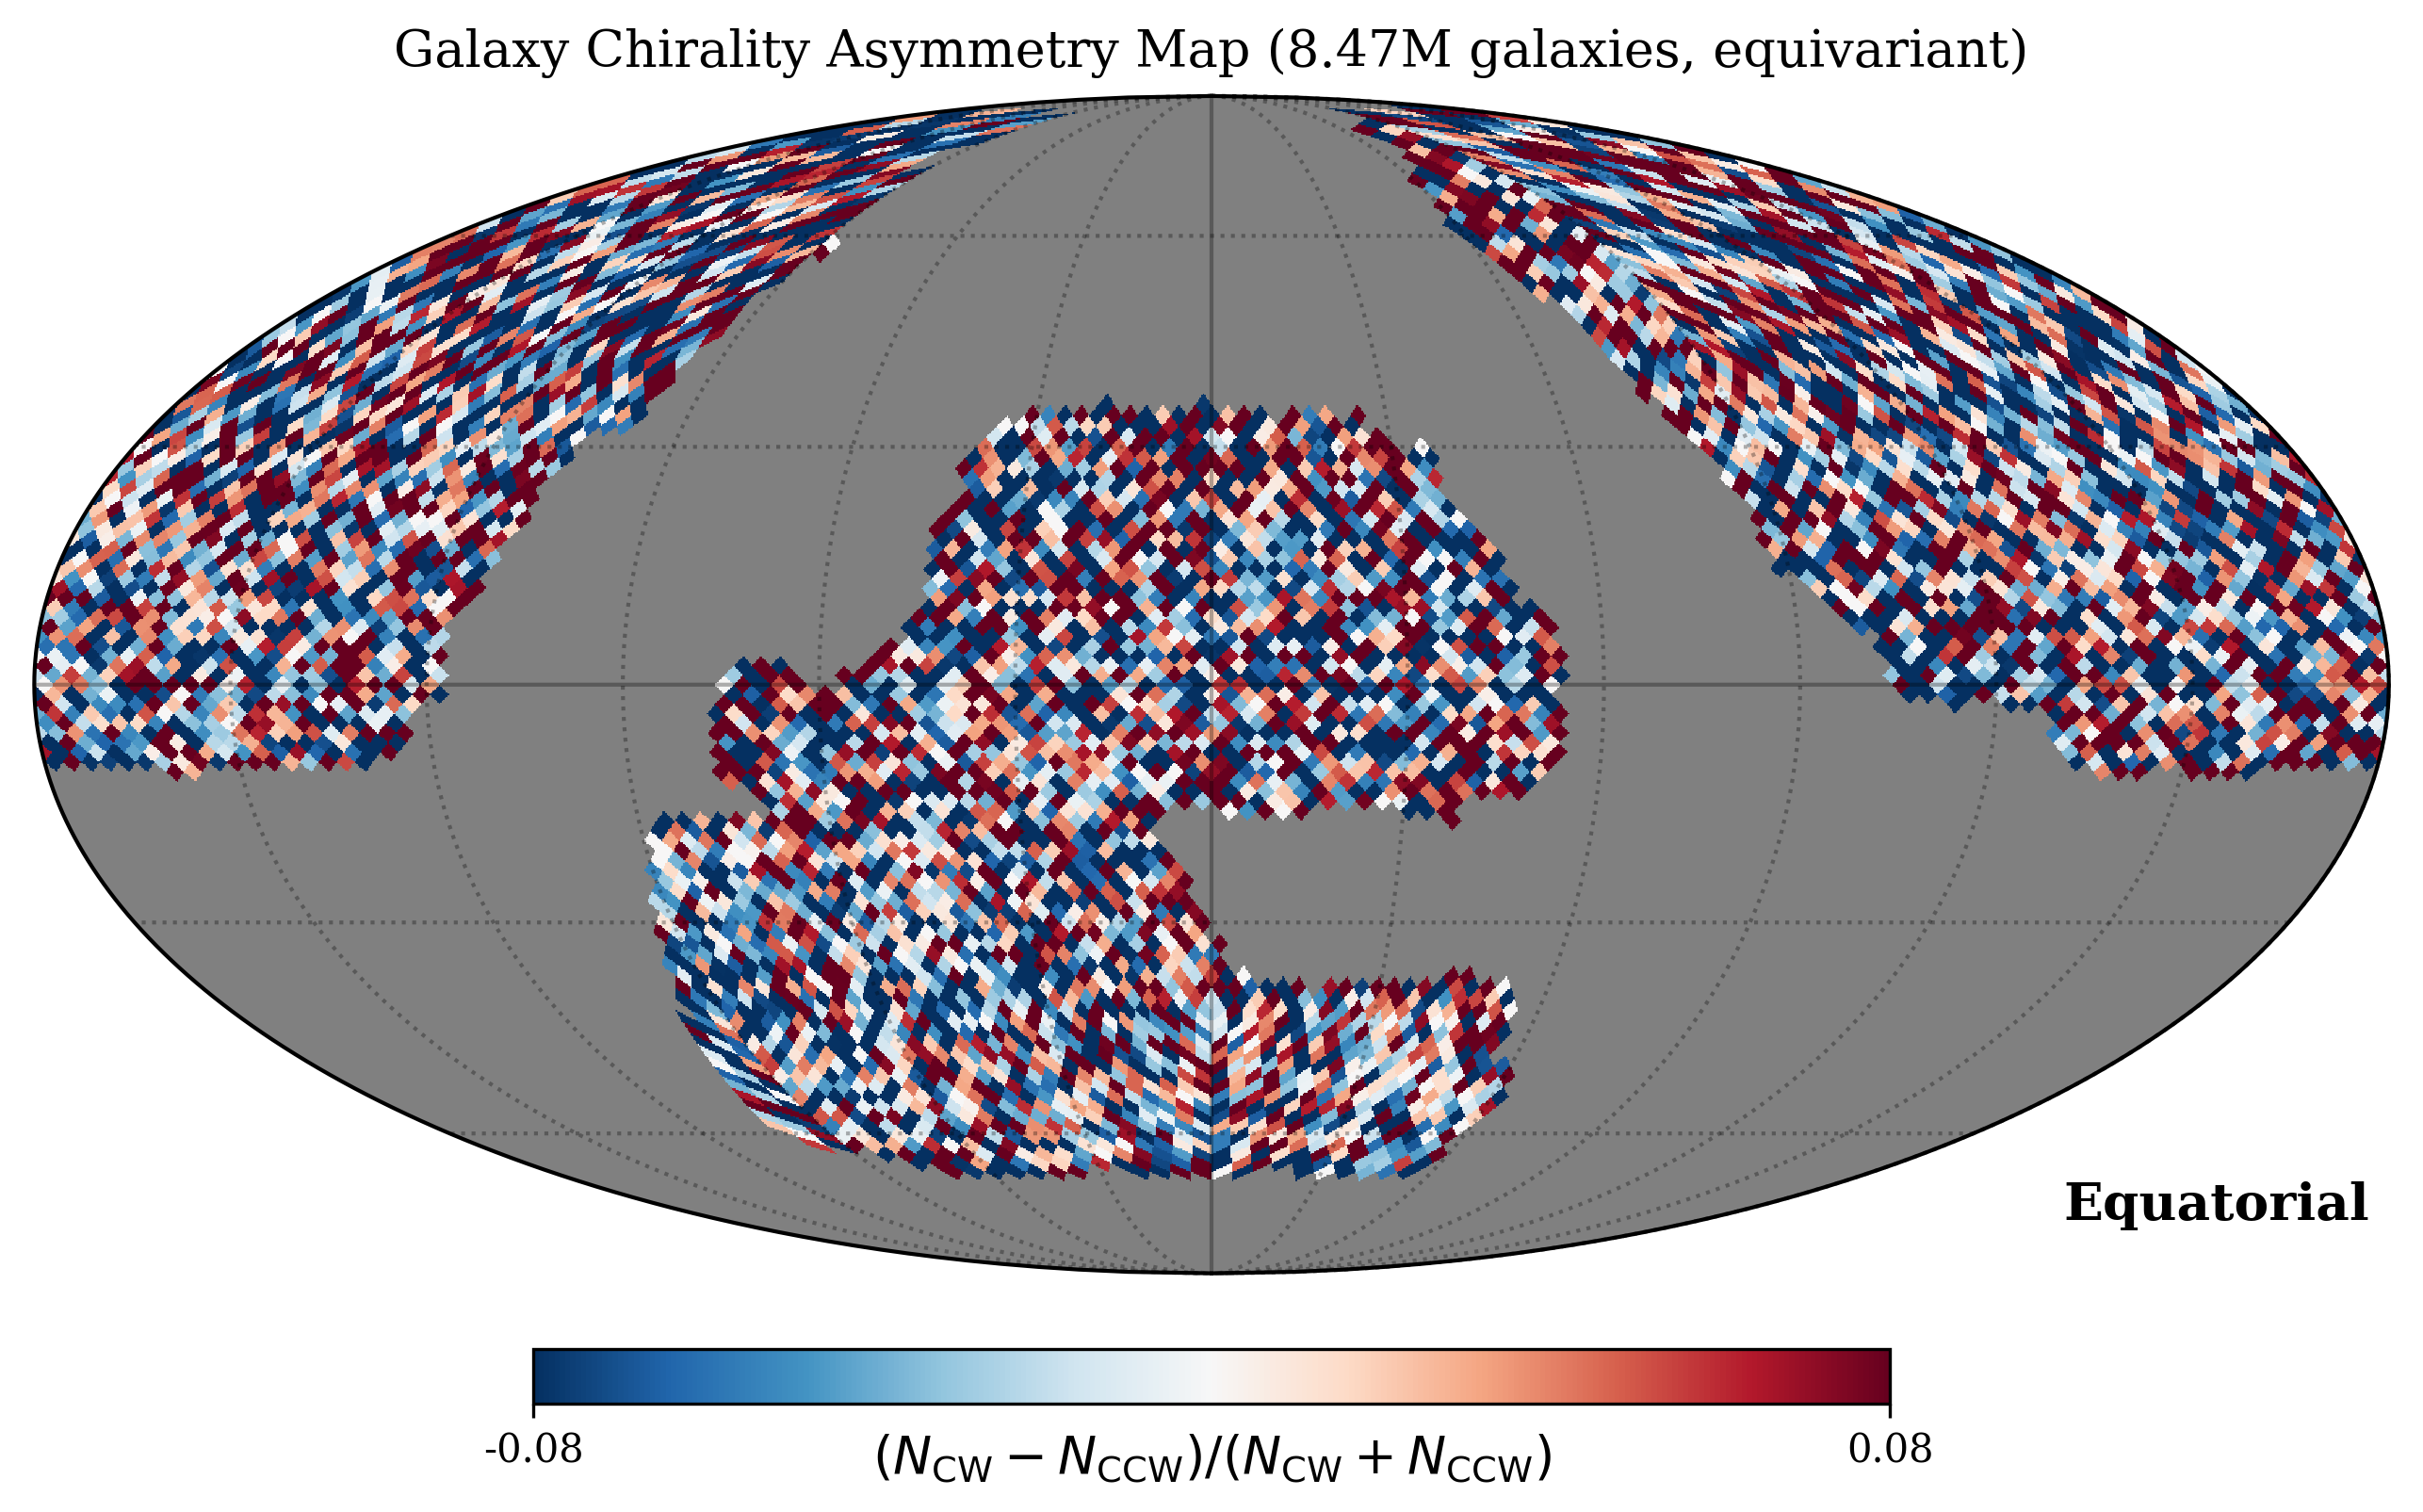
\includegraphics[width=\columnwidth]{fig_sky_map.png}
\caption{\textbf{Equivariant chirality asymmetry map of the full 8.47\,M-galaxy
catalog} (Mollweide projection, equatorial coordinates; per-pixel asymmetry
$A_p=(N_{\rm CW}-N_{\rm CCW})/(N_{\rm CW}+N_{\rm CCW})=2(f_{{\rm CW},p}-\tfrac12)$
at HEALPix $\nside=64$, color scale $[-0.08,+0.08]$) on the 24,087-pixel
\FSC{} support ($f_{\rm sky}=0.49005$; Sec.~\ref{sec:catalog_schema}). This
is the full-catalog map, a broader footprint than the 23,633-pixel,
887,472-galaxy \HCRI{} support used for the primary dipole fit below; no
coherent large-scale structure is visually apparent in either support.}
\label{fig:skymap}
\end{figure}

To make this null quantitative against a specific alternative amplitude, we
use a coverage-calibrated observed-label injection--recovery: signal
injections at fixed pixel occupancy on 2,000 isotropically random axes per
amplitude are passed through the exact committed primary estimator and the
exact committed $10^4$-draw null. Recovered detection probability rises
monotonically with amplitude (e.g.\ $0.24$ at $A=0.40\%$, $0.91$ at
$0.90\%$, saturating to unit coverage by $1.5\%$) and crosses $95\%$
coverage at
\begin{equation}
A_{95}^{\rm obs}\simeq0.98\%\quad(\text{full-amplitude, observed-label}),
\label{eq:a95_obs}
\end{equation}
i.e., $A_{95}^{\rm obs}$ is a \emph{detection-power} threshold: the
amplitude at which an injected signal, run through the exact primary
estimator and null, is recovered at $\geq\!95\%$ power. It is not itself a
confidence-level bound on the measured value. The committed null
distribution's own $95$th percentile, $0.669\%$
(\artifact{research/bh\_universe\_dipole/a95\_null\_cl\_2026\_09\_02.py}), is
also not a confidence-level bound on $A_{\rm dip}$: it is the same
no-signal acceptance boundary already reported as the rank test above
($p=0.238$), restated as a critical value rather than a rank -- values of
$A_{\rm dip}$ at or above $0.669\%$ occur in fewer than $5\%$ of null
draws, which is a statement about the null, not an interval on the true
amplitude. A genuine $95\%$ confidence-level upper limit requires the
complementary Neyman inversion: the largest injected amplitude $A$ whose
recovered-amplitude distribution keeps the observed $A_{\rm
dip}=0.4665\%$ above its own $5$th percentile. Running the same committed
injection model and estimator used for Eq.~\ref{eq:a95_obs}, but recording
the $5$th (not the $50$th/$84$th) percentile of \texttt{recovered\_amp}
per injected amplitude and inverting against $A_{\rm dip}$, gives
\begin{equation}
A_{95}^{\rm CL}\simeq0.75\%\quad(\text{full-amplitude, Neyman 95\% CL}),
\label{eq:a95_cl}
\end{equation}
(bracketed between $0.75\%$, $p_5=0.466\%$, and $0.80\%$, $p_5=0.493\%$;
\artifact{research/bh\_universe\_dipole/a95\_upper\_limit\_2026\_09\_02.py},
2,000 random-axis injections per amplitude, same estimator/support/null as
Eq.~\ref{eq:a95_obs}). The observed $A_{\rm dip}=0.467\%$ lies below this
genuine $95\%$ CL upper limit, below the detection-power floor
$A_{95}^{\rm obs}=0.98\%$, and below the null's own $95$th-percentile
critical value $0.669\%$. $A_{95}^{\rm obs}$ and $A_{95}^{\rm CL}$ are
additionally both \emph{observed-label} statements on the classifier's
chirality labels, not physical parity-amplitude bounds on deprojected
spin: the physical bound additionally requires a
spatially resolved morphology transfer function, which remains an open gate
in the archived release paper~\cite{Golden:P4v274}. This distinction
matters directly for Sec.~\ref{sec:bh}, which uses Eq.~\ref{eq:a95_obs} as
the sensitivity floor against which the black-hole-universe claim is
confronted.

A distinct harmonic diagnostic on the wider, 24,087-pixel \FSC{} support
(Fig.~\ref{fig:skymap}) gives a fixed-occupancy $\ell=1$ moment
$z=+6.923$ (add-one rank $p=0.001996$ on 500 draws; a separate
binomial-monopole null gives $+6.983$ at 500 draws and $+7.207$ at $10^4$
draws). This diagnostic uses a different support, estimator (NaMaster
MASTER-decoupled harmonic power, not the real-space uniform-pixel dipole
fit), and null family than the primary \HCRI{} result above, and does not
by itself overturn the primary null: the archived release attributes it to
classifier- and footprint-systematic structure rather than a
dipole-aligned axis, on the strength of the classifier-injection forward
model (Sec.~\ref{sec:catalog_classifier}) and a battery of
declination/RA/equal-area partition checks~\cite{Golden:P4v274}. Full
weighted-least-squares and GZ1 human-vote diagnostics are retained as
systematics cross-checks in the archived release and are not repeated
here.

\begin{figure}[t]
\centering

\includegraphics[width=\columnwidth]{fig_injection_recovery.png}
\caption{Observed-label injection--recovery curve underlying
Eq.~\ref{eq:a95_obs}: recovered one-sided detection probability
($p<0.05$ against the exact committed $10^4$-draw null) vs.\ injected
full-amplitude $A$, on 2,000 isotropically random axes per amplitude, run
through the exact committed primary \HCRI{} estimator. The curve crosses
$95\%$ coverage at $A_{95}^{\rm obs}=0.98\%$ (red dotted); the observed
amplitude $A_{\rm dip}=0.467\%$ (green dash-dot) sits well inside the
sub-detection-power region. Plotted directly from the committed
\artifact{pipelines/p2\_chirality/analysis/a95\_observed\_label\_upper\_limit\_v1\_0\_265.json}
(no re-inference).}
\label{fig:injrecovery}
\end{figure}

\begin{center}
\footnotesize
\begin{tabular}{rr@{\hspace{1.2em}}rr}
\toprule
$A$ (\%) & Det.\ frac. & $A$ (\%) & Det.\ frac. \\
\midrule
$0.40$ & $0.236$ & $0.96$ & $0.947$ \\
$0.50$ & $0.348$ & $0.98$ & $0.950$ \\
$0.60$ & $0.533$ & $1.00$ & $0.954$ \\
$0.70$ & $0.675$ & $1.10$ & $0.982$ \\
$0.80$ & $0.818$ & $1.20$ & $0.998$ \\
$0.90$ & $0.911$ & $1.50$ & $1.000$ \\
\bottomrule
\end{tabular}
\end{center}
Detection fraction is monotonic in injected amplitude across all 18
grid points (2,000 axes each); the tabulated crossing between the $0.96\%$
and $0.98\%$ rows brackets $A_{95}^{\rm obs}$ (linear interpolation
$0.980\%$; a logistic fit to the full curve gives $0.955\%$, consistent to
better than $0.03$ percentage points).

To characterize how the real-space dipole, its nuisance-marginalized
weighted-least-squares (WLS) variant, the global monopole, and the
NaMaster MASTER-decoupled $\ell=1$ power co-vary, the archived release
evaluates all four estimators on one shared $\nside=8$ block bootstrap
($N_{\rm boot}=2{,}000$ resamples, all valid, seed 42, pre-support-cut HC
sample $N=949{,}584$ -- distinct from this paper's own $887{,}472$-galaxy
primary channel, which is the post-support-cut subset). The resulting
correlation matrix, computed directly from
the committed $4\times4$ joint covariance
(\artifact{pipelines/p2\_chirality/outputs/canonical\_provenance/g3\_joint\_estimator\_covariance\_master\_v2.json}),
is
\begin{center}
\footnotesize
\begin{tabular}{lrrrr}
\toprule
 & real-space & WLS & monopole & $C_1^{\rm master}$ \\
\midrule
real-space & $1.000$ & $0.158$ & $-0.037$ & $0.794$ \\
WLS & $0.158$ & $1.000$ & $-0.020$ & $0.129$ \\
monopole & $-0.037$ & $-0.020$ & $1.000$ & $-0.061$ \\
$C_1^{\rm master}$ & $0.794$ & $0.129$ & $-0.061$ & $1.000$ \\
\bottomrule
\end{tabular}
\end{center}
The monopole is the only channel with $|z|>3$ against its own bootstrap
scatter ($z=-6.57$; the FSC harmonic diagnostic above is the same
structure seen through a different estimator, consistent with its
$0.79$ correlation to the real-space channel here); the other three
channels are all non-significant on this same shared bootstrap
($z=+2.21$ real-space dipole, $+0.81$ WLS dipole, $-0.61$ MASTER
$\ell=1$), consistent with the primary null. The block-bootstrap
real-space $z=+2.21$ is a distinct statistic from the primary null's
fixed-occupancy $z_{\rm mom}=+0.635$ (\HCRI{}-support quantity, above): the
former is the full-sample dipole amplitude over its own $\nside=8$
block-bootstrap scatter (which does not model the pixel-occupancy
constraint), the latter is the fixed-occupancy label-randomization
statistic reported as the primary result; both are non-significant and
neither supersedes the other. The monopole is nearly
uncorrelated with the other three; the primary real-space dipole and its
WLS variant are only weakly correlated ($0.16$), consistent with them
answering related but non-identical questions on different supports.

% ============================================================
\section{Void/non-void environment contrast}
\label{sec:void}
% ============================================================

A second, independent probe tests whether classifier-labelled chirality
depends on large-scale environment, using the released DESIVAST
void catalog~\cite{DESIVAST:2025} intersected with the DR1 companion of the
catalog in Sec.~\ref{sec:catalog}. The DESIVAST GALZONE TARGET universe
($694{,}642$ unique TARGETIDs) joined against the catalog yields $145{,}789$
rows; retaining the $145{,}766$ rows with \texttt{OUT}$=0$ as the quality
parent, $31{,}937$ fall inside the union of released VoidFinder holes
(``void'') and $113{,}829$ do not (``non-void'').
\begin{center}
\footnotesize
\begin{tabular}{lr}
\toprule
Stage & $N$ \\
\midrule
DESIVAST GALZONE TARGET universe & $694{,}642$ \\
$\quad\to$ joined against the chirality catalog & $145{,}789$ \\
$\quad\to$ quality parent (\texttt{OUT}$=0$) & $145{,}766$ \\
$\qquad$ void (VoidFinder hole union) & $31{,}937$ \\
$\qquad$ non-void & $113{,}829$ \\
\bottomrule
\end{tabular}
\end{center}
The focal fit is an unpenalized Newton--Cholesky logistic MLE on a
declared $13$-column linear nuisance basis (void indicator,
linear redshift, magnitude, log-size, classifier confidence, extinction,
imaging leg, morphology, and the GALZONE edge flag standing in for coarse
sky blocks), with cluster-robust (CR1) inference on $50$ occupied
$\nside=4$ HEALPix clusters; a null-imposed Rademacher wild-cluster
efficient-score test provides a second, non-asymptotic inference path on
the same clustering. The basis was declared after review and inspection of
the data and is exploratory, not preregistered. It gives an adjusted
non-void-minus-void contrast
\begin{equation}
\Delta f_{\rm CW} = +0.00145\,,\quad \mathrm{SE}=0.00332\ (\mathrm{cluster\text{-}sandwich})\,,
\label{eq:void_contrast}
\end{equation}
$95\%$ CI $[-0.00504,+0.00795]$, two-sided normal $p=0.661$; a null-imposed
99,999-draw Rademacher wild-cluster efficient-score test gives $p=0.673$.
Both results are null-consistent: classifier-labelled spiral chirality shows
no significant dependence on void/non-void environment in this sample. This
test is exploratory and post-hoc (the void/non-void hierarchy was fixed
after inspecting the data) and is reported as a catalog-specific
non-detection for classifier labels, not a physical-handedness or
cosmological constraint. A secondary, four-class cosmic-web diagnostic
(T-Web; Fig.~\ref{fig:voidbar}) on 812,793 env-labelled rows
(Void $N=428$, Wall $N=6{,}673$, Filament $N=408{,}187$, Cluster
$N=397{,}505$) shows the same
pattern -- no significant CW-fraction trend from void through wall,
filament, to cluster; the Void bin's small $N$ limits its statistical
power relative to the other three classes; author-constructed VoidFinder and the Tempel and ASTRA
web classifications are retained as further secondary diagnostics in the
archived companion study and are not repeated here.

\begin{figure}[tbp]
\centering
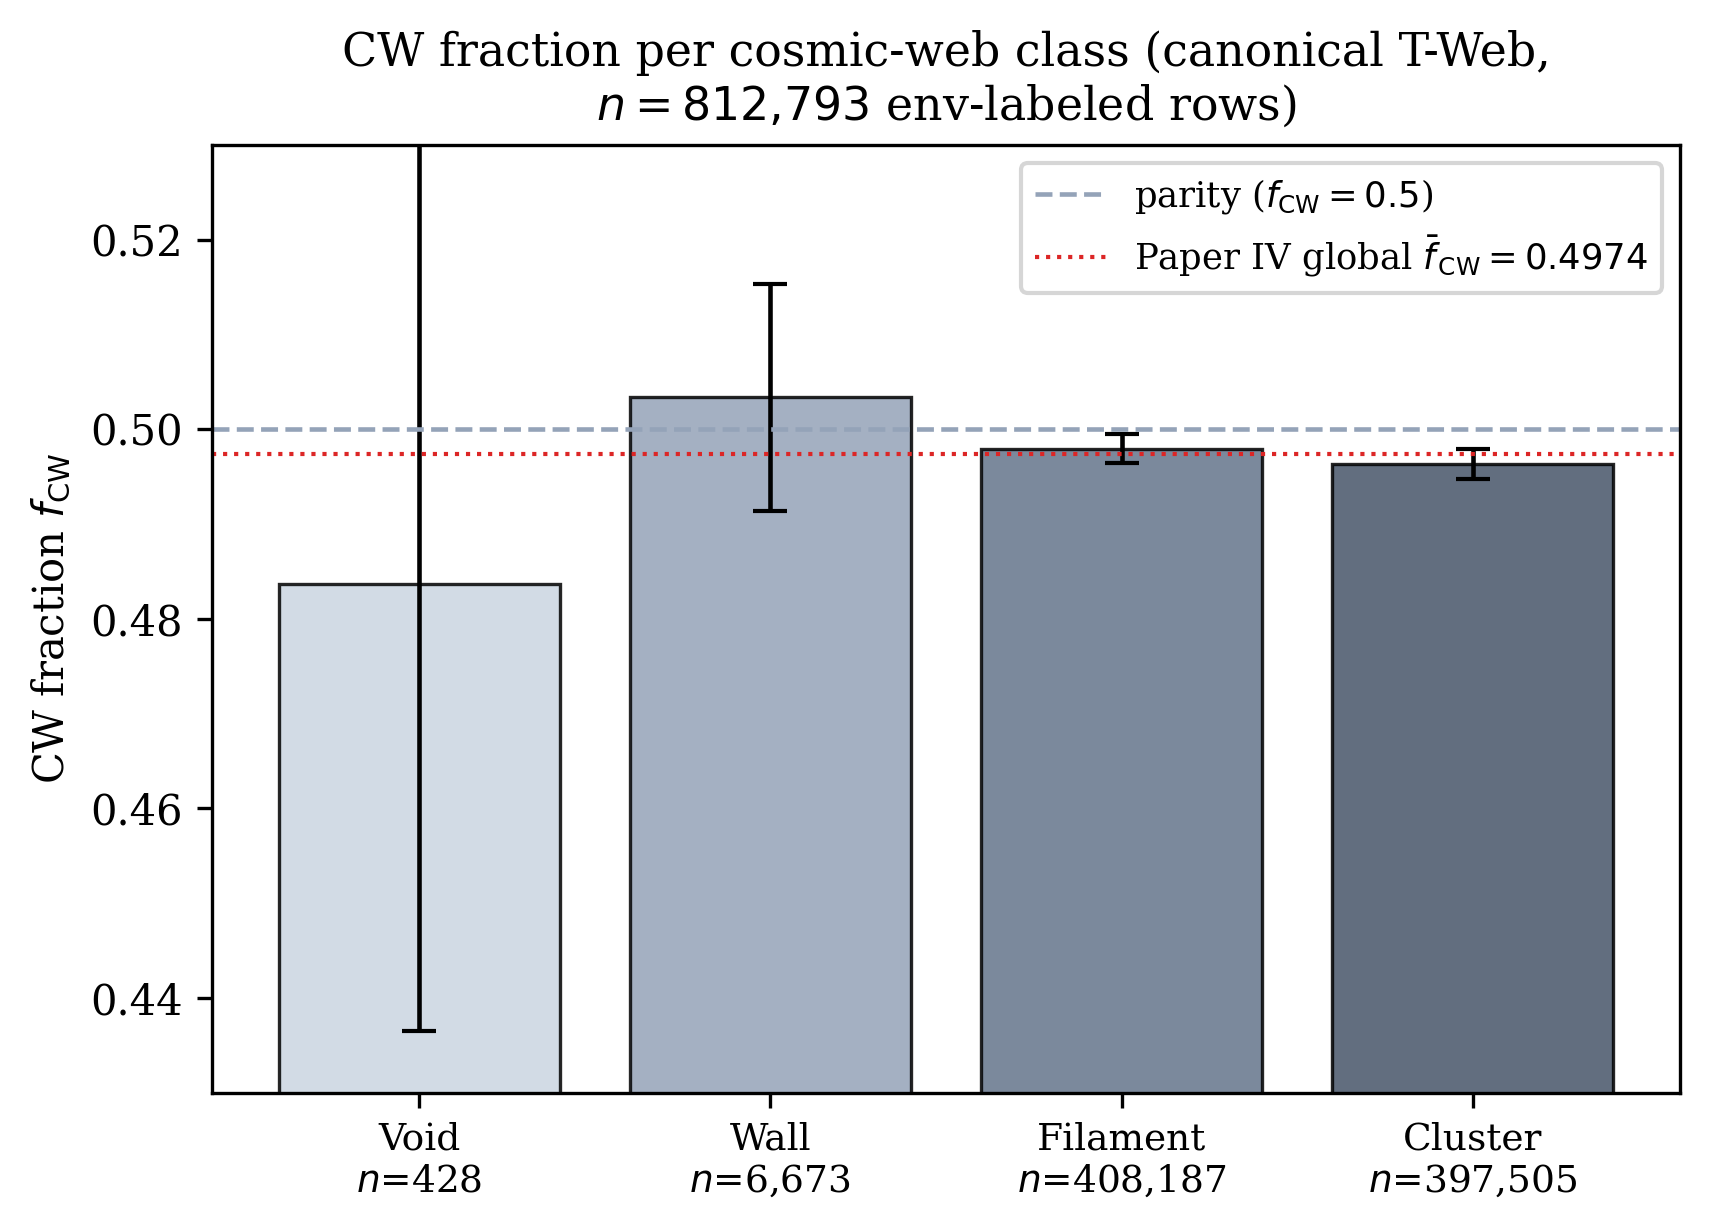
\includegraphics[width=\columnwidth]{fig_p5_cw_by_env_bar.png}
\caption{Secondary diagnostic: classifier-labelled CW fraction per T-Web
cosmic-web class (Void/Wall/Filament/Cluster) on 812,793 env-labelled rows
(Sec.~\ref{sec:void}). This four-class T-Web run is a secondary cross-check;
the primary void/non-void DESIVAST result (Eq.~\ref{eq:void_contrast}) uses
the two-category VoidFinder-hole membership test, not this classification.
The Filament ($\bar f_{\rm CW}\approx0.4980$) and Cluster
($\bar f_{\rm CW}\approx0.4958$) bars sit slightly off the reference line at
different offsets; both are consistent with the same catalog-wide residual
monopole discussed in Sec.~\ref{sec:catalog_classifier}, not an
environment-dependent chirality effect (both are within a few tenths of a
percentage point of the 0.4974 reference and neither individually clears
the null threshold used in the primary contrast).}
\label{fig:voidbar}
\end{figure}

\subsection{Robustness: clustering scale and void-definition sensitivity}
\label{sec:void_robust}

The focal contrast (Eq.~\ref{eq:void_contrast}) clusters standard errors on
$\nside=4$ HEALPix superpixels. Repeating the identical $N=145{,}766$,
$13$-column fit and contrast at $\nside=2$ and $\nside=8$, and separately
clustering by the $3{,}750$ nearest VoidFinder-MAXIMALS 3-D clusters, holds
the point estimate fixed at $+0.00145$ throughout while the $95\%$ CI
half-width varies mildly with the clustering scale: $\nside=2$
$[-0.00622,+0.00912]$, $\nside=4$ (focal) $[-0.00504,+0.00795]$, $\nside=8$
$[-0.00496,+0.00787]$, and the 3-D-cluster scheme $[-0.00476,+0.00767]$ --
every interval contains zero. A separate, wider sensitivity family repeats
the void/non-void contrast under three void-finding algorithms spanning two
algorithmic families -- VoidFinder (sphere-growing) and the ZOBOV/V2
watershed as V2-REVOLVER and V2-VIDE -- plus two catalog-native GALZONE
zone definitions, five correlated statistics in total, none of which
approaches the Bonferroni-5 per-test threshold ($|z|\leq1.25$ across all
five rows against $|z|^{\rm Bonf}_{0.05,5}\approx2.58$); the simultaneous
descriptive interval across all five, inflated to hold jointly at
family-wise $95\%$ confidence, has a maximum half-width of $0.75$
percentage points and remains centered near zero. Full per-algorithm tables
and the catalog-native GALZONE construction are in the archived companion
study~\cite{Golden:P5v147}. We report one multiplicity note across this
paper's three headline tests (the primary real-space dipole,
Sec.~\ref{sec:dipole}; the DESIVAST void/non-void contrast,
Sec.~\ref{sec:void}; and the T-Web four-class diagnostic above): none is
independently significant at even an uncorrected $\alpha=0.05$, so no
multiple-comparison correction changes the qualitative null verdict on any
of the three.

% ============================================================
\section{The black-hole-universe prediction and its exclusion}
\label{sec:bh}
% ============================================================

\subsection{What the model predicts}
\label{sec:bh_predicts}

Poplawski's mechanism papers~\cite{Poplawski:2010,Poplawski:2012,Poplawski:2016}
establish that Einstein--Cartan torsion, sourced by fermion spin, generates
a repulsive spin--spin contact interaction that grows faster than the
attractive curvature term at high density, halting collapse before a
singularity and driving a bounce into an expanding daughter universe inside
the black hole's interior. Poplawski~(2010)~\cite{Poplawski:2010} first
proposes torsion as an alternative to inflation for generating a nonsingular
early universe; Poplawski~(2012)~\cite{Poplawski:2012} develops the
spinor--torsion coupling that produces a nonsingular bounce; Poplawski~(2016)~\cite{Poplawski:2016}
extends the mechanism specifically to a universe originating inside a black
hole, arguing the Einstein--Cartan interior bounces into an expanding
daughter universe rather than terminating in a singularity. None of these
three mechanism papers addresses rotation or a preferred axis for the
daughter universe -- they establish only that the bounce itself occurs.
Poplawski~(2020)~\cite{Poplawski:2020} extends this picture: if the parent
black hole is rotating, its spin axis defines a preferred, non-inertial
axis for the daughter universe, and ``galaxies tend to align their axes of
rotation with the preferred axis, resulting in clockwise-counterclockwise
asymmetry.'' This is the paper's only statement connecting the model to an
observable galaxy-spin signature. We read it in full and find \emph{no
computed dipole amplitude, alignment fraction, or relaxation timescale}
anywhere in it or in the mechanism papers it builds on: the claim is
qualitative -- a preferred axis exists, and galaxies tend toward it -- not
quantitative. No torque strength, relaxation timescale, or coupling
constant is given from which an amplitude could in principle be derived
without further modeling assumptions beyond what the cited papers state.

To confront the model with data at all, a quantitative closure must be
supplied that the cited literature does not provide. We adopt the minimal
one: let $\eta\in[0,1]$ be the fraction of galaxies whose spin has
relaxed toward the preferred axis, and take the resulting population-level
observed dipole amplitude as
\begin{equation}
A_{\rm pred} \approx \eta\,,
\label{eq:bh_dipole_prediction}
\end{equation}
i.e., full alignment ($\eta=1$) would produce a maximal observed dipole and
no alignment ($\eta=0$) none, linearly in between. Equation~\ref{eq:bh_dipole_prediction}
is \emph{not} derived from Poplawski's papers -- it is the simplest closure
under which the model becomes falsifiable by a dipole measurement, made
explicit here because the alternative is to leave the claim untestable.

\subsection{Confrontation with the observed-label sensitivity floor}
\label{sec:bh_exclusion}

Under Eq.~\ref{eq:bh_dipole_prediction}, $\eta$ is exactly the quantity
Eq.~\ref{eq:a95_obs} bounds: the catalog's coverage-calibrated $95\%$
sensitivity upper limit excludes
\[
\eta > A_{95}^{\rm obs} \simeq 0.98\%
\]
at $\geq\!95\%$ coverage on the primary channel. We compare this floor
against the amplitudes reported in the literature that motivates the model
in the first place, using the committed, deterministic script
\artifact{research/bh\_universe\_dipole/poplawski\_dipole\_exclusion\_2026\_09\_02.py}
(numpy only; no fitting, no randomness; every output is a literal input or a
closed-form function of inputs). Table~\ref{tab:bh_exclusion} lists the
result: every literature amplitude that has been offered as evidence for a
preferred spin axis (Longo 2011; Shamir 2012, 2020, 2022, 2025) exceeds
$A_{95}^{\rm obs}$ by a factor of $2$--$20$ at face value. The present
catalog's $887{,}472$-galaxy \HCRI{} supported-pixel sample is $4$--$3{,}400\times$
larger than every comparison sample in Table~\ref{tab:bh_exclusion} except
Shamir (2022)'s same-survey DESI Legacy sample ($N=1.3$ million), which is
larger than the primary channel. Under the committed script's illustrative
observed-to-physical bridge $g=0.398$ (Assumption~2 below; not an
established calibration), the two lowest-amplitude, largest-$N$ rows --
Shamir (2020) and same-survey Shamir (2022), both $2$--$4\%$ -- drop below
$A_{95}^{\rm obs}$ (\texttt{exceeds\_A95\_obs\_after\_g\_bridge=false} in the
committed output json); the other three rows remain above it under the
bridge. We do not use this bridge to strengthen the exclusion (Assumption~2);
we report it because it weakens the exclusion for exactly the two claims
made on the largest comparison samples, and that should not go unstated.

\begin{deluxetable}{lrrr}[!htbp]
\tablewidth{\columnwidth}
\tablecaption{Literature spin-axis amplitude claims vs.\ $A_{95}^{\rm obs}=0.98\%$
(Eq.~\ref{eq:a95_obs}). Ratio is the claim's low-end amplitude over
$A_{95}^{\rm obs}$; all exceed 1, i.e.\ all lie above this catalog's
detection-power floor at face value (two of five drop below it under the
illustrative $g=0.398$ bridge; \S\ref{sec:bh_exclusion}). The table's five
rows pool four non-commensurable statistic families -- Longo's dipole amplitude, Shamir (2012)'s
per-bin asymmetry, Shamir (2020/2022)'s global asymmetry fraction, and
Shamir (2025)'s clockwise:counterclockwise count ratio, each from a distinct
label space (visual/algorithmic handedness classification vs.\ the Ganalyzer
algorithm vs.\ a small-$N$ visual/algorithmic count) -- against this paper's
observed-label ViT+TTA amplitude; the ratio column is not a like-for-like
statistical comparison across rows. Computed by
\artifact{research/bh\_universe\_dipole/poplawski\_dipole\_exclusion\_2026\_09\_02.py}.
\label{tab:bh_exclusion}}
\tablehead{\colhead{Source} & \colhead{Amplitude} & \colhead{$N$} & \colhead{Ratio}}
\startdata
Longo 2011~\cite{Longo:2011} & $\sim\!7\%$ & 15,158 & $7.1$ \\
Shamir 2012~\cite{Shamir:2012} & $5$--$20\%$ & 127,000 & $5.1$ \\
Shamir 2020~\cite{Shamir:2020} & $2$--$4\%$ & 200,000 & $2.0$ \\
Shamir 2022~\cite{Shamir:2022DESI} & $2$--$4\%$ & 1,300,000 & $2.0$ \\
Shamir 2025~\cite{Shamir:2025JWST} & $20$--$33\%$ & 263 & $20.4$ \\
\enddata
\end{deluxetable}

\subsection{Exclusion statement}
\label{sec:bh_statement}

Under the closure of Eq.~\ref{eq:bh_dipole_prediction}, the DESI Legacy DR8
catalog's coverage-calibrated observed-label sensitivity disfavors, at
$\geq\!95\%$ detection power (not a confidence-level exclusion; a genuine
$95\%$ CL statement is given in Sec.~\ref{sec:dipole}), any preferred-axis
alignment mechanism that would produce an observed-label dipole above
$\sim\!1\%$ on this sample -- a factor of $2$--$20$ below the amplitudes the
model's own observational motivation reports at face value
(Table~\ref{tab:bh_exclusion}), though two of those amplitudes, on the two
largest comparison samples, drop below the floor under the (not adopted for
strengthening) illustrative bridge. This statement rests on five explicit
assumptions:

\begin{enumerate}[leftmargin=*,itemsep=1pt]
\item The closure $A_{\rm pred}\approx\eta$ (Eq.~\ref{eq:bh_dipole_prediction})
is adopted for lack of a quantitative prediction in the cited Poplawski
papers; a first-principles closure would require a computed relaxation
timescale and torque strength that do not exist in the literature we could
locate.
\item $A_{95}^{\rm obs}$ is an \emph{observed-label} sensitivity floor
(classifier-labelled chirality), not a physical parity-amplitude bound on
deprojected spin. The observed-to-physical bridge requires the spatially
resolved morphology transfer function, an open gate in the archived catalog
paper; an illustrative bridge factor $g=0.398$ used there for a different
comparison is explicitly not an established calibration and is not used to
strengthen this statement.
\item The preferred axis is a free direction in the model (inherited from
an unobserved parent black hole); \texttt{healpy.fit\_dipole} fits both
amplitude and direction, which is the correct match to a model with no
predicted axis. This analysis, like the tests in
Secs.~\ref{sec:dipole}--\ref{sec:void}, tests amplitude only (a full-sky
real-space dipole and a void/non-void contrast), not a search matched to a
specific predicted axis.
\item The committed script also reports an illustrative $1/\sqrt{N}$
sensitivity-floor ansatz calibrated to this catalog's own anchor point,
used only to compare statistical reach across sample sizes; it is not a
re-derivation of any other paper's estimator, mask, or null and is not the
basis of the Ratio column in Table~\ref{tab:bh_exclusion}.
\item Literature amplitude ranges are reported as published, with no
re-analysis of their pipelines performed here (cross-reference only, as in
Iye \etal~\cite{Iye:2021} and Patel \& Desmond~\cite{Patel:2024}). Shamir
(2025)'s $20$--$33\%$ is that paper's reported clockwise:counterclockwise
count-ratio range (${\sim}2$:$1$ to $1.5$:$1$), not an asymmetry fraction
in the same sense as the other rows (Table~\ref{tab:bh_exclusion} caption).
\end{enumerate}

We emphasize what this section does \emph{not} claim: it does not test, and
is not evidence for or against, the nonsingular matter-bounce cosmology this
research program otherwise develops from the same torsion mechanism (that
line derives an early-universe non-Gaussianity signature, not a late-time
galaxy-spin observable, and stands or falls on its own evidence). It tests
only Poplawski's black-hole-universe model's one stated observational
consequence, under the minimal closure that makes that consequence testable
at all.

% ============================================================
\section{Discussion}
\label{sec:discussion}
% ============================================================

Two independent probes on this catalog -- a full-sky real-space dipole
(Sec.~\ref{sec:dipole}) and a void/non-void environment contrast
(Sec.~\ref{sec:void}) -- are both null-consistent. Neither reaches the
$2$--$33\%$ amplitudes reported by Shamir and collaborators, nor
Longo's $\sim\!7\%$ claim; both are consistent instead with the independent
reanalyses of Iye, Yagi \& Fukumoto (2021)~\cite{Iye:2021}, who found no
significant dipole in Shamir's own SDSS catalog after correcting known
systematics, and Patel \& Desmond (2024)~\cite{Patel:2024}, who found
consistency with isotropy across every public spin-classification dataset to
within $3\sigma$. At $8{,}474{,}531$ total catalog objects, this is the largest single catalog
release brought to the question; the $887{,}472$-galaxy primary
supported-pixel test is itself larger than every comparison sample in
Table~\ref{tab:bh_exclusion} except Shamir (2022)'s same-survey $1.3$-million-galaxy
DESI Legacy catalog. Its detection-power floor (Eq.~\ref{eq:a95_obs}) is
$2$--$20\times$ tighter, at face value, than the amplitudes the disputed
claims report (Table~\ref{tab:bh_exclusion}).

Section~\ref{sec:bh} adds the piece the literature comparison alone does
not supply: a direct confrontation with the theoretical claim that motivates
testing spin-axis alignment in the first place. The result is a genuine,
if qualified, exclusion -- qualified because Poplawski's papers do not
themselves commit to a quantitative amplitude, so the exclusion binds a
minimal closure of the claim rather than a number the model's author
derived. We regard that as the honest state of the test: the model predicts
a direction of effect (preferred-axis alignment) that this catalog is
well-positioned to detect were it present at the amplitudes the
observational literature has claimed, and does not detect it.

% ============================================================
\section{Conclusions}
\label{sec:conclusions}
% ============================================================

We release an 8,474,531-object DESI Legacy DR8 chirality catalog and report
two independent, large-sample null tests of a preferred galaxy-spin axis:
a primary real-space dipole ($N_{\rm support}=887{,}472$;
$z_{\rm mom}=+0.635$, $p=0.238$; $A_{95}^{\rm obs}\simeq0.98\%$) and a
DESIVAST void/non-void environment contrast ($N=145{,}766$;
$\Delta f_{\rm CW}=+0.00145$, $p=0.66$). Reading Poplawski's rotating
black-hole-universe papers in full, we find the model predicts only a
qualitative preferred-axis alignment tendency, not a computed amplitude;
under the minimal closure that makes the claim testable, our sensitivity
floor disfavors an alignment-driven dipole above $\sim\!1\%$ at
$\geq\!95\%$ detection power, well below the $\sim\!2$--$33\%$ amplitudes
reported in the observational literature the model is invoked to explain.
This confirms, on the largest catalog release assembled for the question,
the independent reanalyses of Iye \etal\ (2021) and Patel \& Desmond
(2024). We make no claim beyond this stated test: the
result bears on the black-hole-universe model's spin-axis prediction only,
not on the separate matter-bounce cosmology this research program develops
from the same torsion mechanism.

\appendix

% ============================================================
\section{Supplementary systematics diagnostics}
\label{sec:app_systematics}
% ============================================================

This appendix condenses the systematics checks the archived release uses
to attribute the \FSC{} harmonic residual (Sec.~\ref{sec:dipole}) to
classifier- and footprint-level structure rather than a dipole-aligned
axis, restoring self-containedness beyond the primary channel's own
null result.

\textbf{Sample-purity ladder.} Stratifying the full spiral sample by
equivariant max-class probability into five confidence bins, a
$+3.29\sigma$ excess appears in the $1.87$M-galaxy $[0.5,0.6)$ bin under a
confidence-stratified dipole estimator and null; this signal does not
survive the sample-purity cut used for the primary channel ($p_{\rm
eq}>0.6$ gives $-0.03\sigma$ under the same statistic). This is a distinct
diagnostic from the primary \HCRI{} real-space dipole and illustrates why
the release adopted the high-confidence cut as the primary science sample
rather than the full spiral catalog.

\textbf{Fixed-support multipole vector.} On the checksummed 24,087-pixel
\FSC{} support, the binary-mask fixed-occupancy null gives the multipole
vector $z_{\ell=1,\ldots,5}=(+6.923,+2.931,+3.089,-0.317,+1.606)$: only
$\ell=1$ is a $>5\sigma$ outlier, and its rank-$p$ significance
($p=0.001996$, Sec.~\ref{sec:dipole}) does not by itself distinguish a
primordial dipole from a low-$\ell$ classifier or footprint systematic,
which is why the release cross-checks with directional partitions.

\textbf{Directional partition checks.} Splitting the \FSC{} support into
four RA quadrants gives per-quadrant dipole deviations ranging from
$-0.82\sigma$ to $+2.49\sigma$ -- scatter, not the consistent projection a
primordial dipole would produce. A Galactic-hemisphere split gives
$\sigma_{\rm iso}=+0.47$ (north, $b>0$) and $+2.02$ (south, $b<0$) against
an independent per-pixel binomial null, consistent with dust-correlated
foreground structure in the south rather than a primordial signal. Seven
equal-spiral-count declination slabs ($N=457{,}308$--$457{,}309$ each) span
$f_{\rm CW}$ deviations of $-0.110\%$ to $-0.463\%$ from $0.5$, all within
$0.5\%$; an independent equal-area declination partition gives a compatible
verdict (deviations up to $0.49\%$ on the full spiral sample, $0.56\%$ on
the HC subsample). All partition checks are consistent with a bounded,
spatially structured residual entering upstream of the classifier
(Sec.~\ref{sec:catalog_classifier}), not a coherent dipole-aligned
gradient.

\textbf{Statistical-only scale reference.} For the full-amplitude dipole
convention $p_{\rm CW}(\hat n)=\tfrac12(1+A\cos\theta)$, the idealized
full-sky Fisher floor at $N_{\rm spiral}=3{,}201{,}160$ is
$\sigma(A)=\sqrt{3/N_{\rm spiral}}=9.7\times10^{-4}$ (a $3\sigma$ ideal
floor of $\approx0.29\%$); this full-sky idealization omits the realized
footprint, classifier transfer, and orientation dependence and is a scale
reference only, not a calibrated detection threshold or a substitute for
the injection-recovery-calibrated $A_{95}^{\rm obs}$ of
Sec.~\ref{sec:dipole}.

% ============================================================
\section*{Data Availability}
% ============================================================

The 8,474,531-row catalog, quarantine, exact null arrays, generator scripts,
and full provenance register are archived under Zenodo DOI
\href{https://doi.org/10.5281/zenodo.21461899}{10.5281/zenodo.21461899}
(concept DOI \href{https://doi.org/10.5281/zenodo.21461898}{10.5281/zenodo.21461898}),
published under CC-BY-4.0, and mirrored at
\url{https://huggingface.co/datasets/bamfai/galaxy-chirality-catalog}. This
is the same archived catalog release used by the sources this paper draws
its quoted numbers from~\cite{Golden:P4v274,Golden:P5v147}. The
black-hole-universe exclusion analysis
(Sec.~\ref{sec:bh}) is fully reproducible from the committed script
\artifact{research/bh\_universe\_dipole/poplawski\_dipole\_exclusion\_2026\_09\_02.py}
and its output
\artifact{research/bh\_universe\_dipole/outputs/poplawski\_dipole\_exclusion\_2026\_09\_02.json}.
Full systematics appendices, harmonic and weighted-least-squares diagnostics,
the classifier bias-hardening audit, and the void/non-void secondary
diagnostic paths (author VoidFinder, T-Web, Tempel, ASTRA) are not
reproduced in this condensed manuscript; they remain available in the
archived source papers~\cite{Golden:P4v274,Golden:P5v147} referenced above.
The catalog is a single Apache Parquet file (952,115,239 bytes for the
pinned source revision) with one row per DESI Legacy DR8 galaxy: a
\texttt{dr8\_id} identifier, sky coordinates, the observed chirality label
(\CW/\CCW/\NS), per-class probabilities, and quality-control flags
including \texttt{raw\_flip\_qc\_unsafe}; a separate quarantine Parquet
contains the 249,066 catalog-wide flagged rows (59,515 within the HC
selection), and a machine-readable schema and validation report accompany
both files at the Zenodo DOI and Hugging Face mirror above. This
manuscript's own version, \paperVersion{} (dated \paperTimestamp), is the
pin for its numbers: it is served alongside its git-tracked source at
\url{https://github.com/Hubify-Projects/bigbounce/blob/main/pipelines/p4prime_chirality_test/paper/main.tex},
and the underlying catalog/quarantine/null-array revision it draws from is
independently pinned by the versioned Zenodo DOI
10.5281/zenodo.21461899 above.

% ============================================================
\section*{Software, Facilities, and Acknowledgements}
% ============================================================

\textit{Software:} NumPy, healpy, HEALPix, NaMaster (pymaster), PyTorch, pandas, SciPy.
\textit{Facilities:} DESI Legacy Imaging Surveys DR8 (data products); no
proprietary telescope time was used in this analysis, which is entirely
based on public archival imaging and catalog data.
\textit{Acknowledgements:} We thank the DESI, DESIVAST, Galaxy Zoo, and
Galaxy Zoo DESI collaborations for public data products without which this
analysis would not be possible.

\begin{thebibliography}{99}

\bibitem{Longo:2011}
M.~J.~Longo,
``Detection of a dipole in the handedness of spiral galaxies with redshifts $z\!\sim\!0.04$,''
Phys.\ Lett.\ B \textbf{699}, 224 (2011), arXiv:1104.2815.

\bibitem{Shamir:2012}
L.~Shamir,
``Handedness asymmetry of spiral galaxies with $z\!<\!0.3$ shows cosmic parity violation and a dipole axis,''
Phys.\ Lett.\ B \textbf{715}, 25 (2012), arXiv:1207.5464.

\bibitem{Shamir:2020}
L.~Shamir,
``Patterns of galaxy spin directions in SDSS and Pan-STARRS show parity violation and multipoles,''
Astrophys.\ Space Sci.\ \textbf{365}, 136 (2020), arXiv:2007.16116.

\bibitem{Shamir:2022DESI}
L.~Shamir,
``Analysis of spin directions of galaxies in the DESI Legacy Survey,''
Mon.\ Not.\ R.\ Astron.\ Soc.\ \textbf{516}, 2281 (2022), arXiv:2208.13866,
DOI:10.1093/mnras/stac2372.

\bibitem{Shamir:2025JWST}
L.~Shamir,
``The distribution of galaxy rotation in JWST Advanced Deep Extragalactic Survey,''
Mon.\ Not.\ R.\ Astron.\ Soc.\ \textbf{538}, 76 (2025), arXiv:2502.18781.

\bibitem{Iye:2021}
M.~Iye, M.~Yagi, and H.~Fukumoto,
``Spin parity of spiral galaxies. III. Dipole analysis of the distribution of SDSS spirals with 3D random walk simulations,''
Astrophys.\ J.\ \textbf{907}, 123 (2021), arXiv:2011.00662.

\bibitem{Patel:2024}
D.~Patel and H.~Desmond,
``No evidence for anisotropy in galaxy spin directions,''
Mon.\ Not.\ R.\ Astron.\ Soc.\ \textbf{534}, 1553 (2024), arXiv:2404.06617.

\bibitem{Poplawski:2010}
N.~J.~Poplawski,
``Cosmology with torsion: An alternative to cosmic inflation,''
Phys.\ Lett.\ B \textbf{694}, 181 (2010), arXiv:1007.0587.

\bibitem{Poplawski:2012}
N.~J.~Poplawski,
``Nonsingular, big-bounce cosmology from spinor-torsion coupling,''
Phys.\ Rev.\ D \textbf{85}, 107502 (2012), arXiv:1111.4595.

\bibitem{Poplawski:2016}
N.~J.~Poplawski,
``Universe in a black hole in Einstein-Cartan gravity,''
Astrophys.\ J.\ \textbf{832}, 96 (2016), arXiv:1410.3881,
DOI:10.3847/0004-637X/832/2/96.

\bibitem{Poplawski:2020}
N.~J.~Poplawski,
``Universe in a rotating black hole and preferred axis,''
arXiv:1910.10819 (preprint, posted October 2019; no journal publication
identified as of this writing -- this is the paper's only source for the
observational preferred-axis claim and the year/identifier mismatch with
its arXiv submission date is stated here explicitly).

\bibitem{Dey:2019}
A.~Dey, D.~J.~Schlegel, D.~Lang \textit{et~al.},
``Overview of the DESI Legacy Imaging Surveys,''
Astron.\ J.\ \textbf{157}, 168 (2019), arXiv:1804.08657.

\bibitem{Walmsley:2023}
M.~Walmsley, C.~Lintott, T.~G{\'e}ron \textit{et~al.},
``Galaxy Zoo DESI: detailed morphology measurements for 8.7M galaxies in the DESI Legacy Imaging Surveys,''
Mon.\ Not.\ R.\ Astron.\ Soc.\ \textbf{526}, 4768 (2023), arXiv:2309.11425.

\bibitem{DESIVAST:2025}
H.~Rinc\'on, S.~BenZvi, K.~A.~Douglass \textit{et~al.},
``DESIVAST: Catalogs of Low-redshift Voids Using Data from the DESI Data
Release 1 Bright Galaxy Survey,'' Astrophys.\ J.\ \textbf{982}, 38 (2025),
DOI:10.3847/1538-4357/adb559, arXiv:2411.00148.

\bibitem{Golden:P4v274}
H.~Golden,
``An Observed-Label Chirality-Dipole Null in 890,069 Quality-Controlled High-Confidence DESI Spirals and an 8.5-Million-Galaxy Catalog,''
v1.0.274 archived release,
Zenodo \href{https://doi.org/10.5281/zenodo.21461899}{doi:10.5281/zenodo.21461899} (2026).

\bibitem{Golden:P5v147}
H.~Golden,
``A Catalog-Native DESIVAST Test of Classifier-Labelled Spiral Chirality in DESI DR1,''
v0.1.147 archived manuscript, served at
\url{https://bigbounce.hubify.app/papers/p5_desi_chirality_v0.1.147-2026-08-03.pdf}
(2026). No independent DOI has been minted for this manuscript as of this
writing.

\bibitem{Golden:P4Zenodo}
H.~Golden,
``Galaxy Chirality Catalog: Archived Release (DESI Legacy DR8, 8,474,531 objects),''
Zenodo (2026), concept DOI
\href{https://doi.org/10.5281/zenodo.21461898}{doi:10.5281/zenodo.21461898}
(same archived release deposit as~\cite{Golden:P4v274}; the dataset and the
release paper are versions of one Zenodo concept record and therefore
intentionally share a DOI family -- the paper cites the specific version
10.5281/zenodo.21461899, the dataset the version-independent concept
10.5281/zenodo.21461898).

\end{thebibliography}

\end{document}
